
%	Conclusion

\section{Future prospects and conclusion}\label{Sec_Conclusion}
\Headerfooter{Future prospects and conclusion}
\subsection{Future prospects}
\vs\hs
Now we continue the observation with a 0.03\% Gd-loaded SK detector, the phase known as SK-VII.
Since the neutron tagging efficiency in SK-VII is higher than that in SK-VI~(35.6\%)~\cite{2023Harada,2022Harada}, more delayed signals can be detected, and the observed number of events can be accumulated faster in SK-VII than in SK-VI.
Figure~\ref{Future_Nmulti} shows the expected $N_{\rm delayed}$ distributions in SK-VII.
In this figure, each bin of the expected $N_{\rm delayed}$ distributions can be estimated as
\begin{eqnarray}
	(N_{\rm delayed} = n) = \sum_{i=n} \{(N_{\rm capture} = i) \times {}_{i}{\rm C}_{n}p^{n}(1 - p)^{i - n}\},
\end{eqnarray}
where $(N_{\rm delayed} = n)$ is the number of events that $N_{\rm delayed} = n$, $(N_{\rm capture} = i)$ is the number of events that $N_{\rm capture} = i$, and $p$ is the neutron tagging efficiency.
Here, the neutron misidentification rate is not considered.
Assuming that the neutron tagging efficiency in SK-VII is 63.0\%~\cite{2023KanemuraSlide}, the statistics (the number of events that $N_{\rm delayed} \geq 1$) increases by about 1.4 times with the same live time as SK-VI.\\
\hs
Figure~\ref{Future_Event_BERT_event} and Figure~\ref{Future_Event_BERT_stat_error} shows the expectation of the observed number of events and the statistical uncertainty as a function of SK-VII live time, respectively.
By combining about three years of data in SK-VII, the statistical uncertainty will be half of this work, and the secondary interaction models will be able to be verified more precisely.\\
\hs
Figure~\ref{Future_Model_Comp_model} shows the expectation of the difference between the observed and expected number of events in $\theta_{\rm C}\in$ [78, 90]~degrees as a function of SK-VII live time.
This difference is estimated using the observed and expected number of events summarized in Table~\ref{tab:obsexp}.
As shown in this figure, BERT is now $\sim$2.2$\sigma$ away from the data.
By combining one year of data in SK-VII, BERT will be more than 3$\sigma$ away from the data.
Furthermore, the evaporation model can be determined at 5$\sigma$ by combining about four years of data in SK-VII.
Once the evaporation model is determined, the secondary interaction uncertainty is reduced, resulting that the systematic uncertainty of measured NCQE cross section is reduced.\\
\hs
Additional measurement using T2K's accelerator neutrino beam interactions in SK-Gd will help further refining the physics models for the secondary interactions.

\begin{figure}[h]
	\centering
	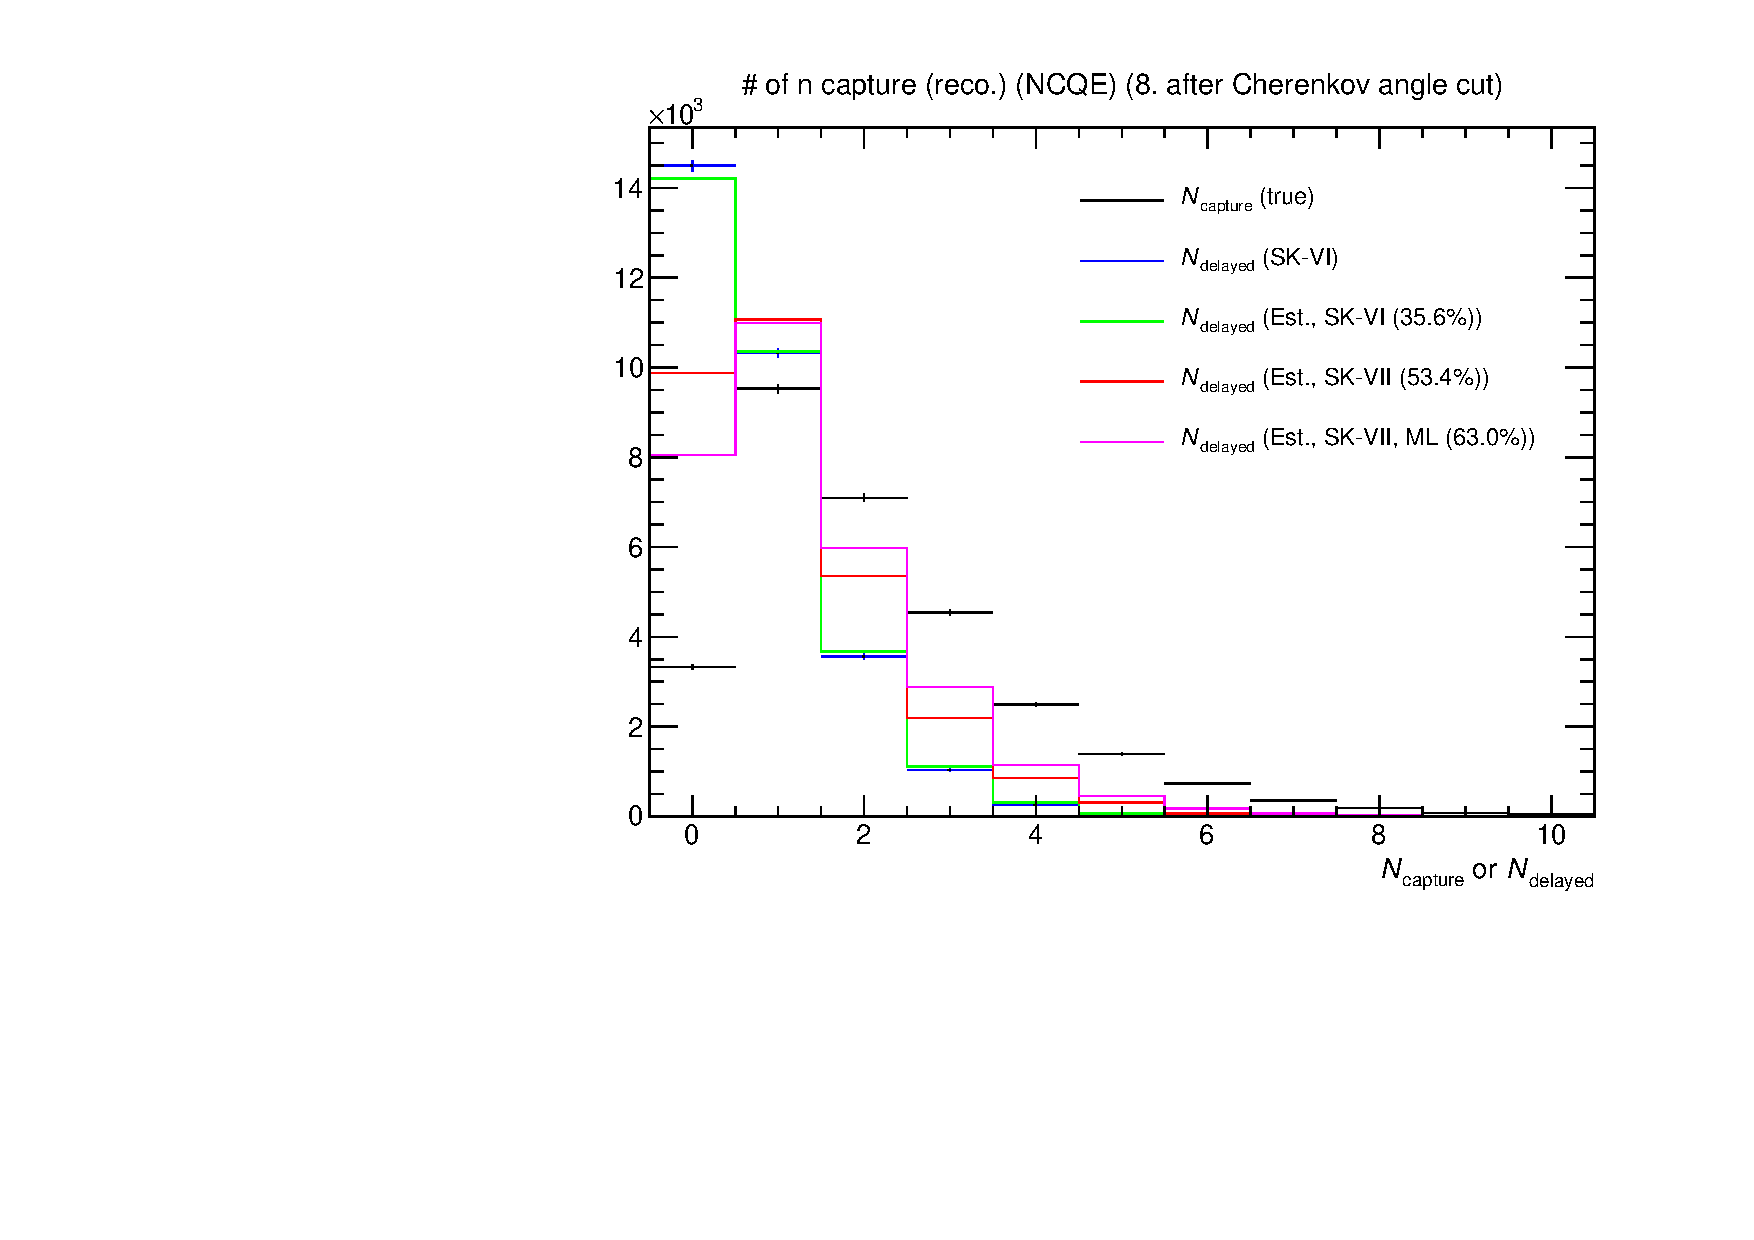
\includegraphics[width=12cm]{PDF/Future/Future_Nmulti}
	\caption[Expected $N_{\rm delayed}$ distributions in SK-VII]{
	Expected $N_{\rm delayed}$ distributions in SK-VII.
	Black plots show the distribution of the number of true neutron captures ($N_{\rm capture}$) before applying neutron tagging without any scalings.
	Blue plots show the $N_{\rm delayed}$ distribution after applying neutron tagging without any scalings in this study.
	Green line, red line, and magenta line show the $N_{\rm delayed}$ distribution estimated from the $N_{\rm capture}$ distribution assuming that neutron tagging efficiency is 35.6\%, 53.4\%, and 63.0\%, respectively.
	35.6\% comes from the neutron tagging efficiency in SK-VI~\cite{2023Harada,2022Harada}.
	53.4\% comes from the assumption that neutron tagging efficiency in SK-VII becomes 1.5 times higher than that in SK-VI~\cite{2023KanemuraSlide}.
	63.0\% comes from the assumption of using the Multi-Layer (ML) neural networks in SK-VII~\cite{2023KanemuraSlide}.
	}\label{Future_Nmulti}
\end{figure}

\begin{figure}[h]
	\centering
%	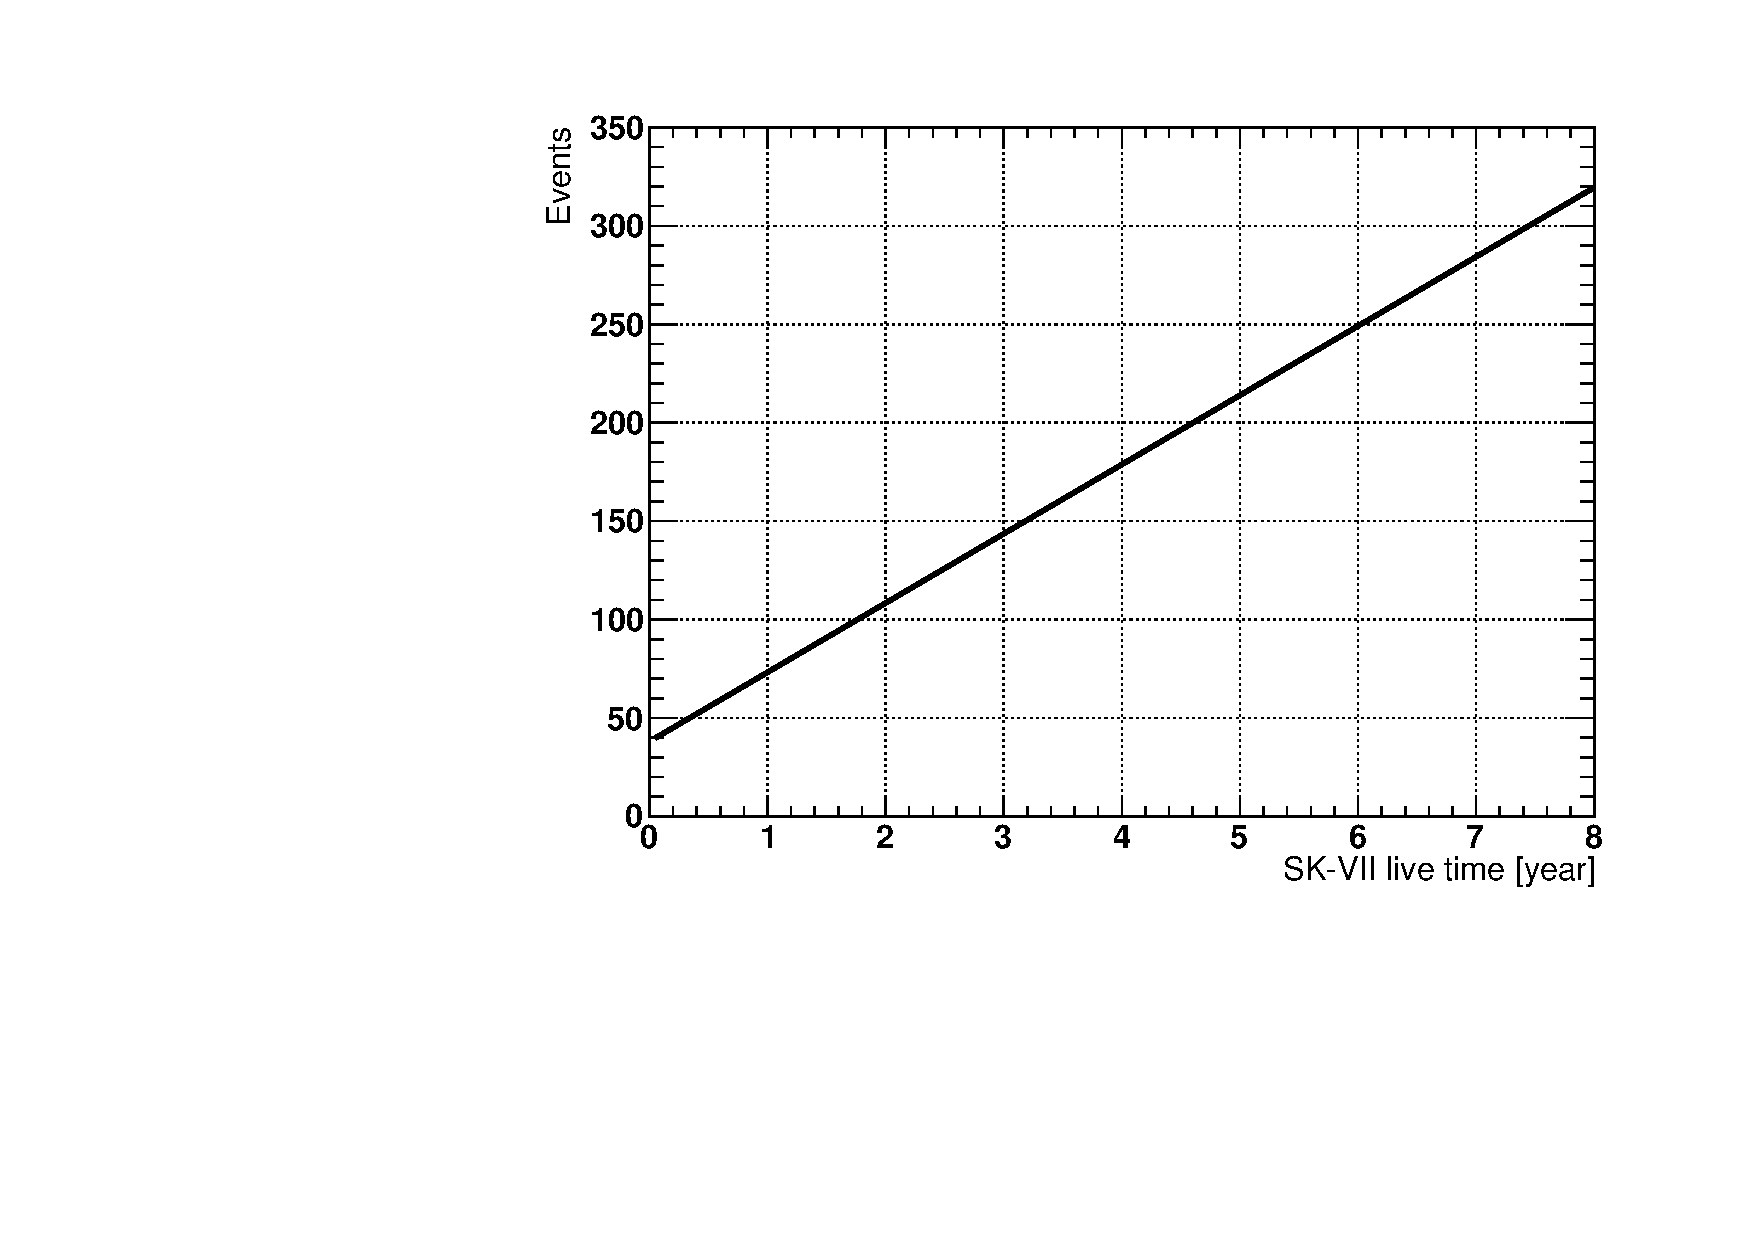
\includegraphics[width=12cm]{PDF/Future_Event/FTFP_BERT_HP/event}
	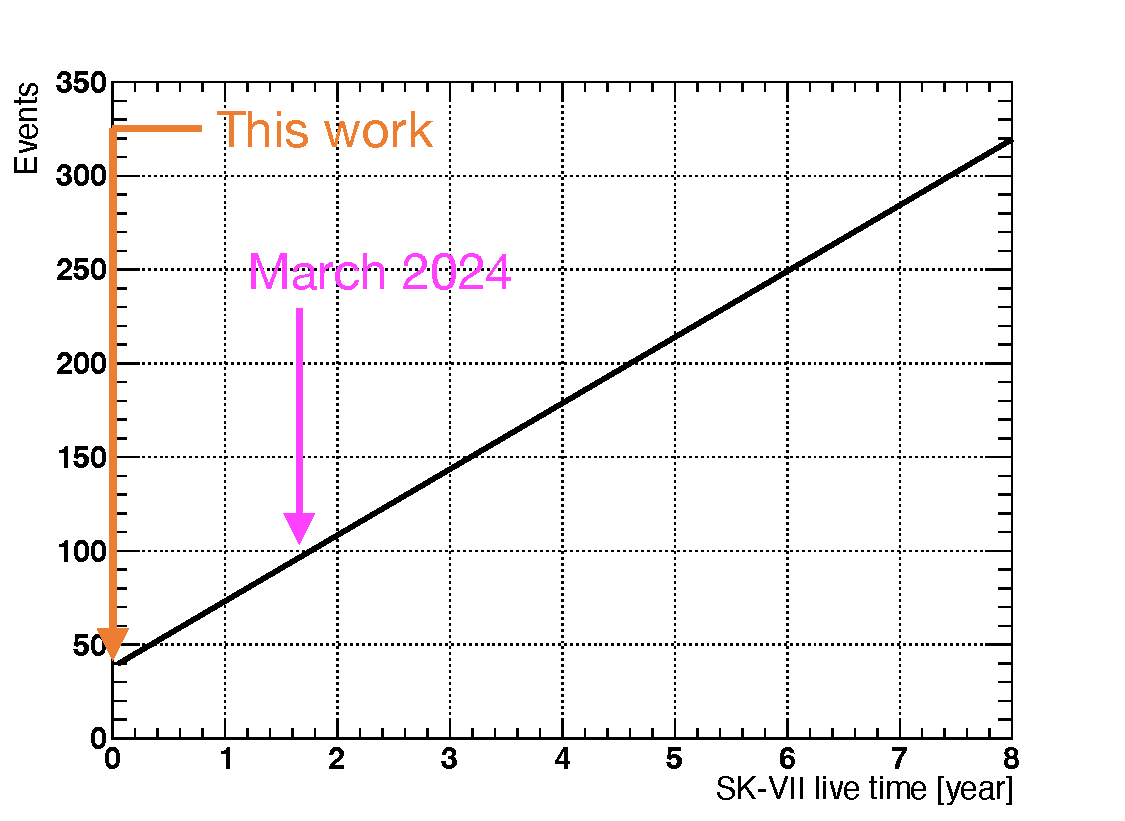
\includegraphics[width=12cm]{Figures/Conclusion/event}
	\caption[Expectation of the observed number of events as a function of SK-VII live time]{
	Expectation of the observed number of events as a function of SK-VII live time.
	Here, it is assumed that the neutron tagging efficiency in SK-VII is 63.0\%~\cite{2023KanemuraSlide}.
	}\label{Future_Event_BERT_event}
\end{figure}

\begin{figure}[h]
	\centering
%	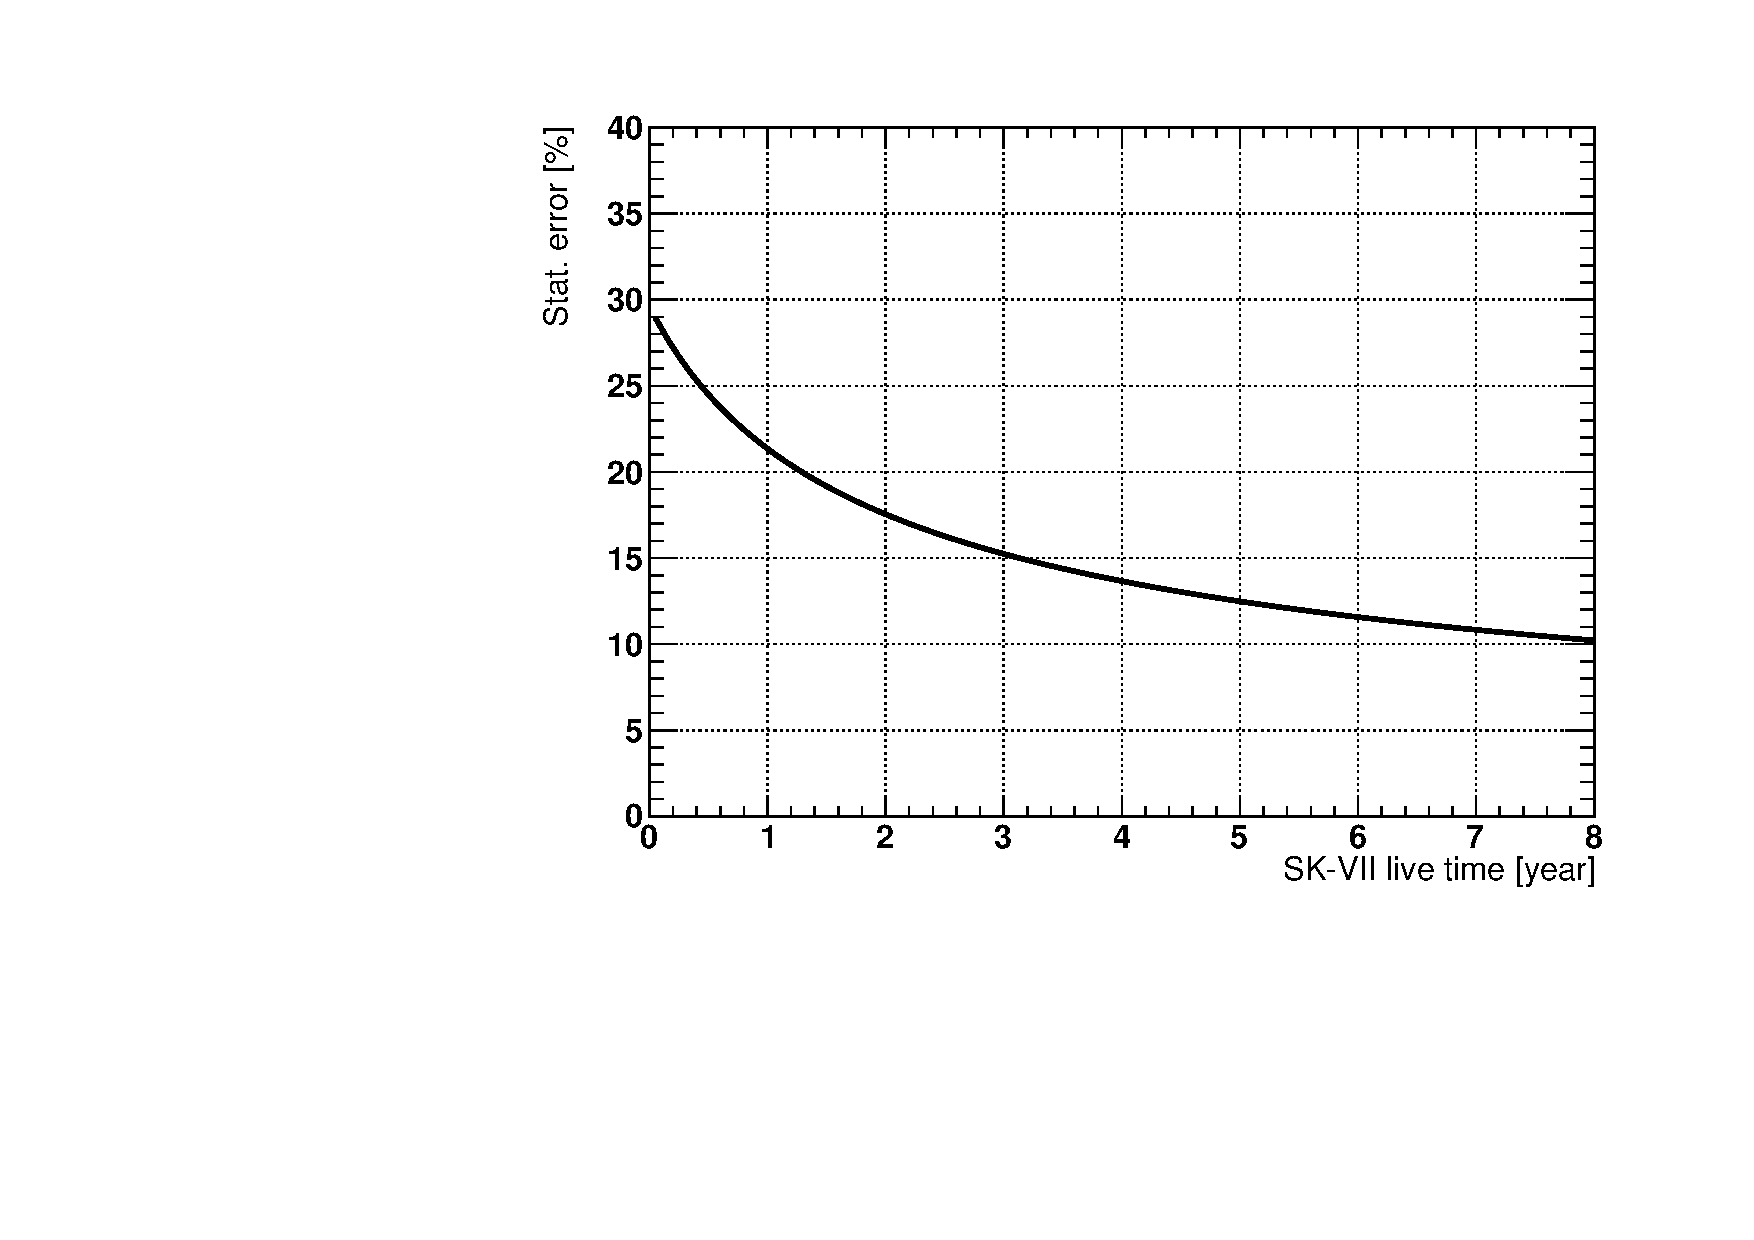
\includegraphics[width=12cm]{PDF/Future_Event/FTFP_BERT_HP/stat_error}
	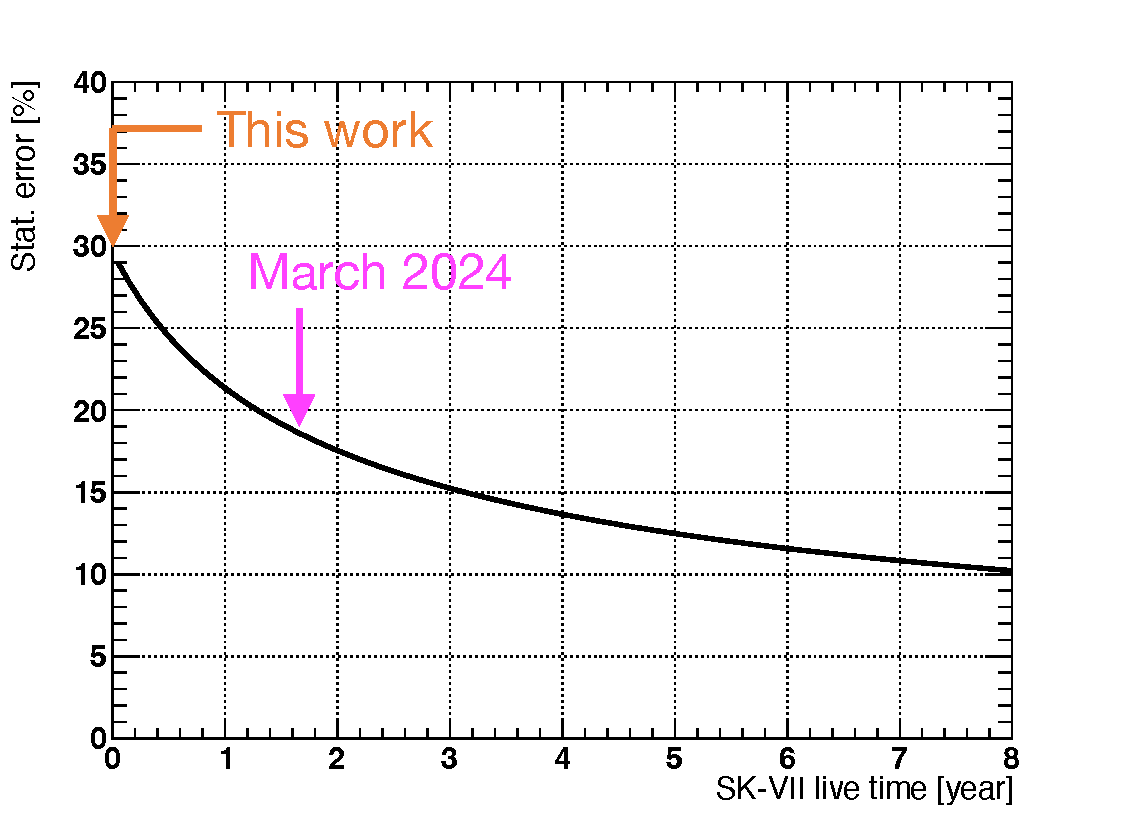
\includegraphics[width=12cm]{Figures/Conclusion/stat_error}
	\caption[Expectation of the statistical uncertainty as a function of SK-VII live time]{
	Expectation of the statistical uncertainty as a function of SK-VII live time.
	Here, it is assumed that the neutron tagging efficiency in SK-VII is 63.0\%~\cite{2023KanemuraSlide}.
	}\label{Future_Event_BERT_stat_error}
\end{figure}

\begin{figure}[h]
	\centering
%	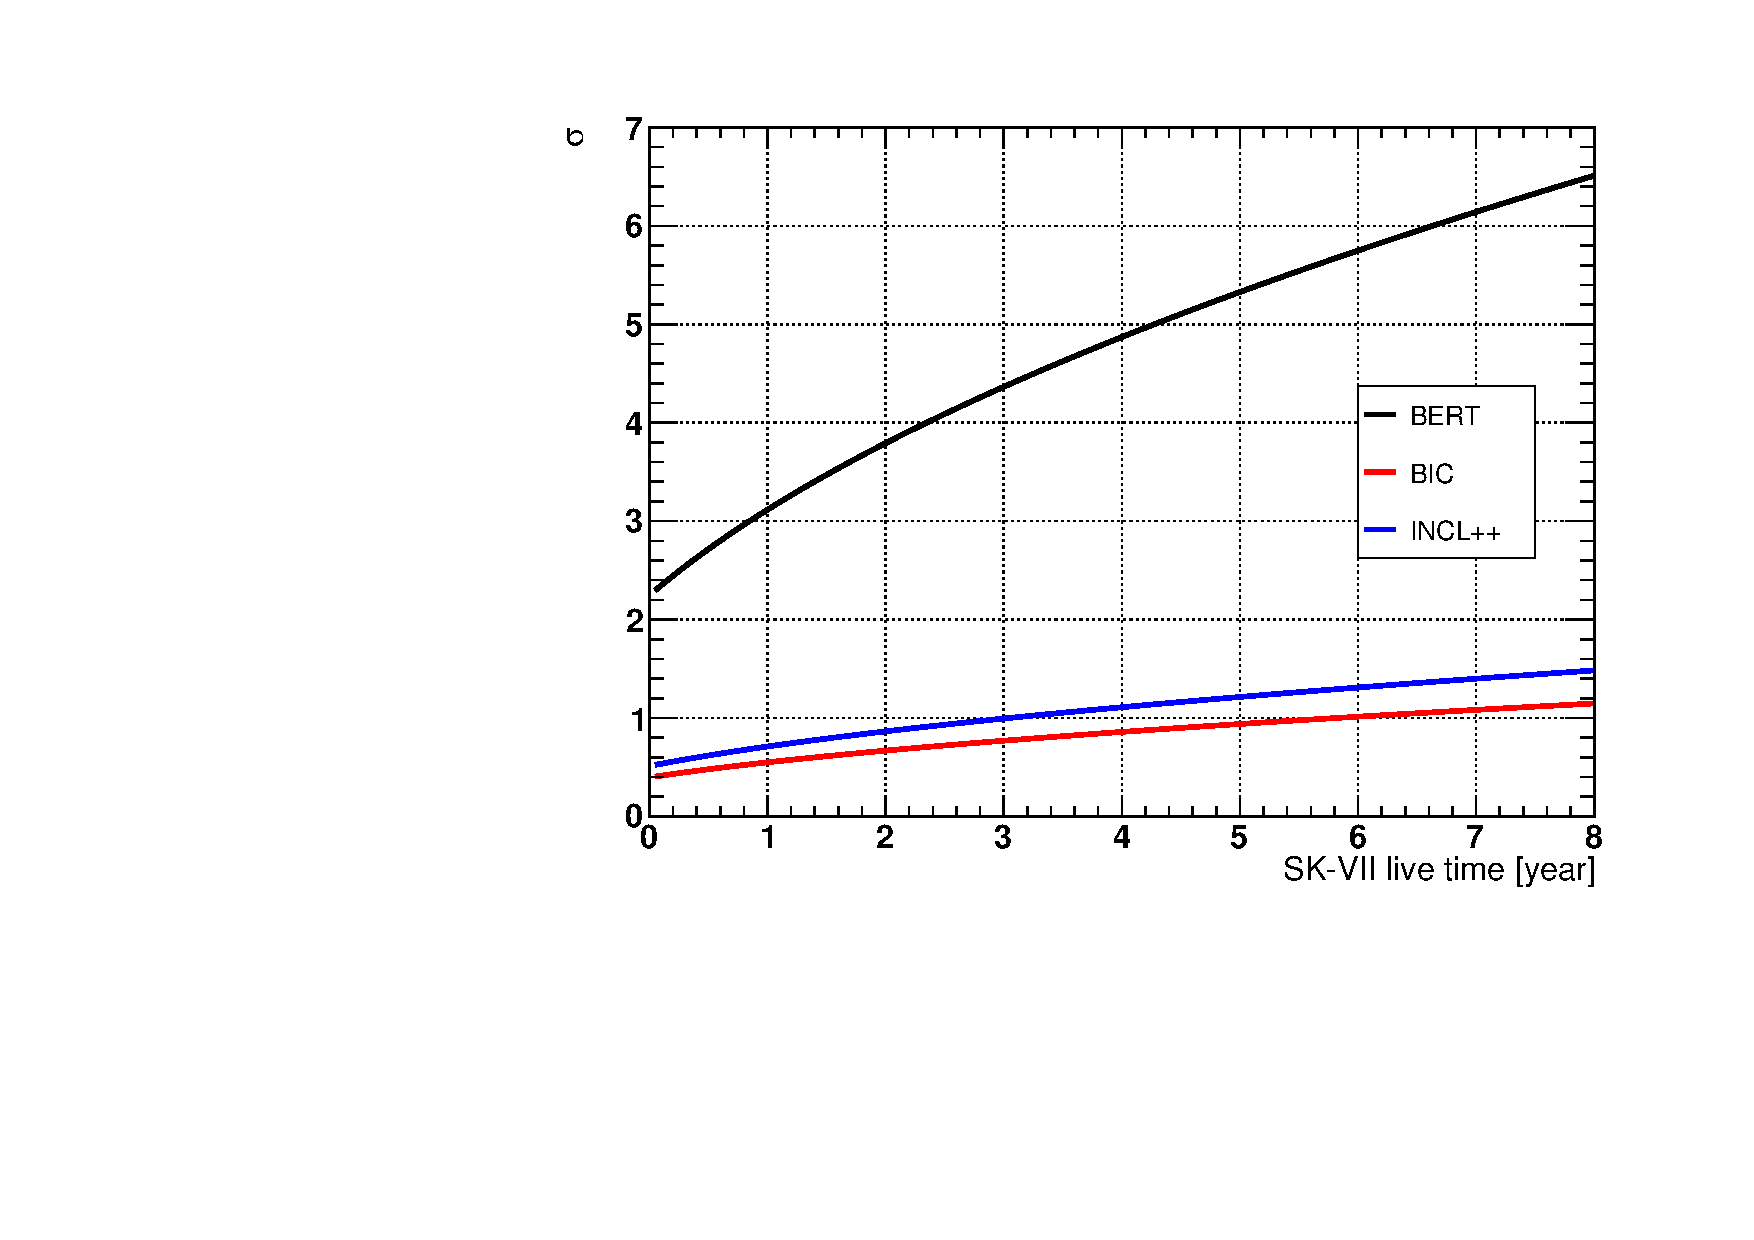
\includegraphics[width=12cm]{PDF/Future_Model/Comparison/model}
	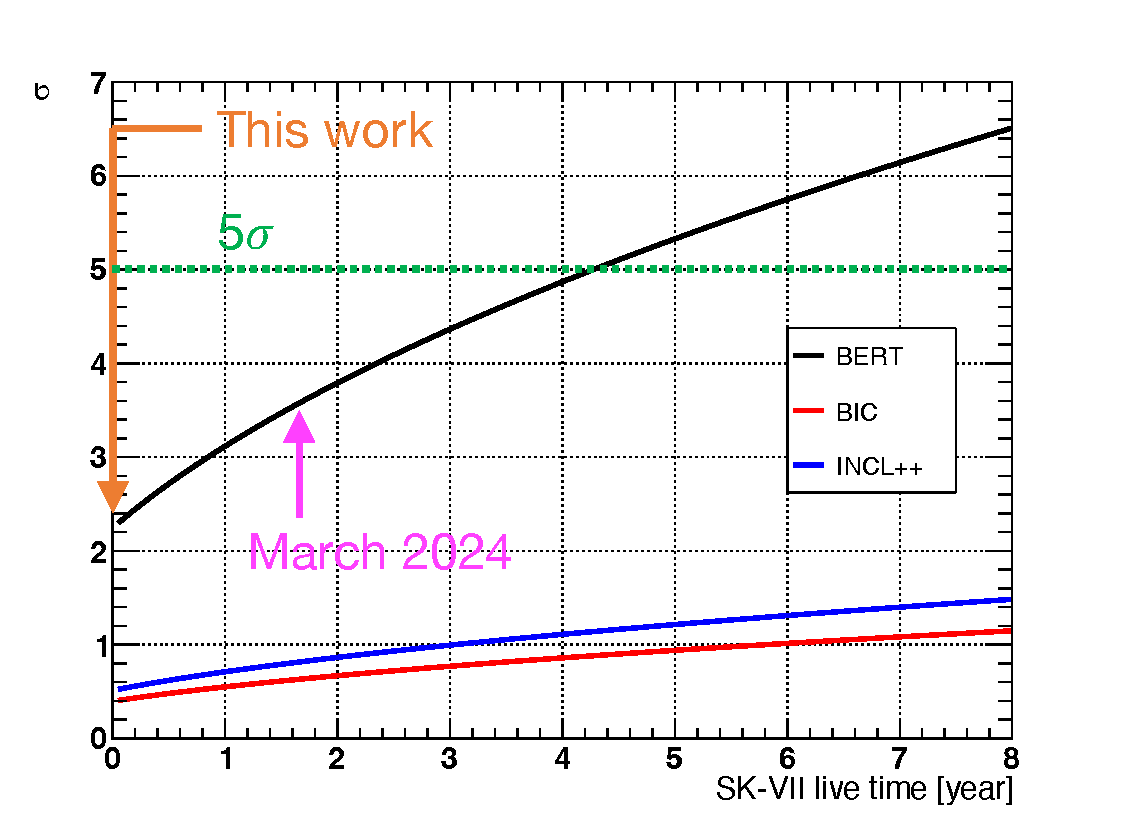
\includegraphics[width=12cm]{Figures/Conclusion/model}
	\caption[Expectation of the difference between the observed and expected number of events in $\theta_{\rm C}\in$ \lbrack78, 90\rbrack~degrees as a function of SK-VII live time]{
	Expectation of the difference between the observed and expected number of events in $\theta_{\rm C}\in$ [78, 90]~degrees as a function of SK-VII live time.
	This difference is estimated using the observed and expected number of events summarized in Table~\ref{tab:obsexp}.
	As for the observed number of events, statistical uncertainty is considered for this estimation.
	As for the expected number of events, systematic uncertainties other than secondary interaction are considered for this estimation.
	Here, it is assumed that the neutron tagging efficiency in SK-VII is 63.0\%~\cite{2023KanemuraSlide}.
	}\label{Future_Model_Comp_model}
\end{figure}





\clearpage

\subsection{Conclusion}
\vs\hs
We performed the comparison of secondary interaction models using atmospheric neutrino events and the measurement of the atmospheric neutrino-oxygen NCQE cross section using 552.2~days of SK-VI data with 0.011\% Gd-loaded water.
Since the backgrounds in this study are the same as those in the DSNB search, event selections in the DSNB search were mainly adopted.
Moreover, since multiple gamma-rays and multiple neutrons are easily emitted in NCQE events, we selected the events that $\theta_{\rm C}$ is greater than 50 degrees and $N_{\rm delayed}$ is greater or equal to one.\\
\hs
After applying all event selections to 552.2 days of SK-VI data, 38 events remained.
In order to understand which secondary interaction model reproduces the observed data, we calculated the chi-square for $\theta_{\rm C}$, $E_{\rm vis}$, and $N_{\rm delayed}$ distributions using the Poisson-likelihood.
As a result, due to the small statistics, the chi-square could not give conclusive results; however, the chi-square values were smaller for BIC and INCL++ than for BERT in all distributions.
The results suggest that the evaporation model used in BIC and INCL++ reproduces the observed data better than that used in BERT.
Furthermore, we measured the atmospheric neutrino-oxygen NCQE cross section using the atmospheric neutrino flux-averaged theoretical NCQE cross section, the observed number of events, and the expected numbers of events.
As a result, the NCQE cross section was measured to be $0.74 \pm 0.22({\rm stat.})^{+0.85}_{-0.15}({\rm syst.}) \times 10^{-38}\,{\rm cm}^{2}/{\rm oxygen}$ in the energy range from 160~MeV to 10~GeV, which was consistent with the atmospheric neutrino flux-averaged theoretical NCQE cross section ($1.02 \times 10^{-38}\,{\rm cm}^{2}/{\rm oxygen}$) and the measured NCQE cross section in the SK pure-water phase ($1.01 \pm 0.17({\rm stat.})^{+0.78}_{-0.30}({\rm syst.}) \times 10^{-38}\,{\rm cm}^{2}/{\rm oxygen}$).
The large systematic uncertainty mainly comes from the difference of secondary interaction models.\\
\hs
Now we continue the observation with a 0.03\% Gd-loaded SK detector, the phase known as SK-VII.
Assuming that the neutron-tagging efficiency in SK-VII is 63.0\%, the statistics increases by about 1.4 times with the same live time as SK-VI, and the statistical uncertainty will be half of this work by combining about three years of data in SK-VII.
Moreover, when we focus on the observed and expected number of events in $\theta_{\rm C}\in$ [78, 90]~degrees, BERT is now $\sim$2.2$\sigma$ away from the data.
By combining about four years of data in SK-VII, the evaporation model can be determined at 5$\sigma$.
Once the evaporation model is determined, the secondary interaction uncertainty is reduced, and the systematic uncertainty of measured NCQE cross section is significantly reduced.





\newpage

